\section{Theorie}
Bei Röntgenstrahlung handelt es sich um durch das Abbremsen von geladenen Teilchen erzeugte elektromagnetische Strahlung mit Energien über $\SI{100}{\electronvolt}$. Elektromagnetische Strahlung lässt sich aufgrund des Superpositionsprinzip als Linearkombination zweier linear polarisierter Wellen beschreiben, die senkrecht zueinander stehen.

\subsection{Röntgenstrahlung an einer Grenzfläche}
Beim Einfall auf eine ebene Grenzfläche, wie in \autoref{fig:fresnel} dargestellt, gilt unter Betrachtung von Röntgenstrahlung für den Brechungsindex eines Mediums
\begin{equation*}
  n = 1 - \delta + i \beta,
\end{equation*}
wobei $\delta$ eine kleine Korrektur in der Größenordnung $10^{-6}$ und $\beta$ die Absorption des Mediums beschreibt.

\begin{figure}[H]
  \centering
  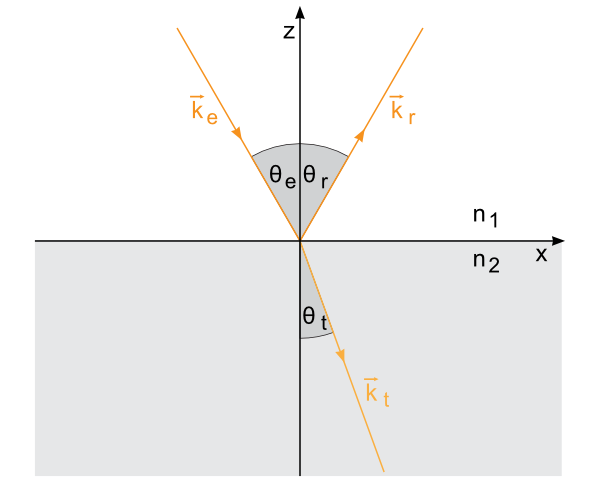
\includegraphics{fresnel.png}
  \caption{Eindimensionale Skizze zur Reflexion und Transmission von elektromagnetischer Strahlung an einer Grenzschicht \cite{fresnel}.}
  \label{fig:fresnel}
\end{figure}

In der Abbildung beschreiben $\vec{k}_\mathrm{e,r,t}$ den Wellenvektor der einfallenden (e), reflektierten (r) und transmittierten (t) Welle und $\theta_\mathrm{e,r,t}$ den jeweiligen Winkel zur Ebene.
Aufgrund des Snellius-Brechungsgesetzes $n_1 \cos {\theta_\mathrm{e}} = n_2 \cos (\theta_\mathrm{a}) $ mit dem Ausfallswinkel $\theta_\mathrm{a}$ gilt $\theta_\mathrm{e} = \theta_\mathrm{r}$. Im Weiteren wird zur Benennung von Winkeln statt $\theta$ der Buchstabe $\alpha$ verwendet.
Die Fresnel-Gleichungen dienen im Allgemeinen zur quantitativen Beschreibung der Amplitudenverhältnisse senkrecht und parallel polarisierten Lichts an einem Grenzmedium. Unter Betrachtung von Röntgenstrahlung sind diese näherungsweise gleich für den parallel und senkrecht polarisierten Teil, da sich die Brechungsindices kaum unterscheiden. Sie lassen sich demnach definieren als

\begin{align*}
  t &= \frac{2 n_1 \sin \alpha_\mathrm{i}}{n_1 \sin \alpha_\mathrm{i} + n_2 \sin \alpha_\mathrm{t}} &
  r &= \frac{ n_1 \sin \alpha_\mathrm{i} - n_2 \sin \alpha_\mathrm{t}}{n_1 \sin \alpha_\mathrm{i} + n_2 \sin \alpha_\mathrm{t}}.
\end{align*}
Handelt es sich nun beim ersten Medium um das Vakuum ($n=1$), so kommt es unter einem kritischen Winkel $\alpha_\mathrm{c}$ zu Totalreflexion, da jeder Brechungsindex von Materie für Röntgenstrahlung $<1$ ist.
Dieser ist näherungsweise gegeben durch
\begin{equation}
  \alpha_\mathrm{c} \approx \sqrt{2\delta} = \lambda \sqrt{\frac{r_e \rho}{\pi}},
  \label{eqn:nocheine}
\end{equation}
wobei $\lambda$ die Wellenlänge der Röntgenstrahlung, $r_e$ der klassische Elektronenradius und $\rho$ die Elektronendichte des Materials sind.
Für die Reflektivität $R = |r|^2$, die das Verhältnis der Intensitäten der reflektierten und einfallenden Welle beschreibt, gilt demnach unter der Annahme $\alpha_\mathrm{i} > 3 \alpha_\mathrm{c}$
\begin{equation}
  R = \left( \frac{\alpha_\mathrm{c}}{2 \alpha_\mathrm{i}} \right)^4.
  \label{eqn:fresnel}
\end{equation}

\subsection{Multischichtsysteme}
\begin{figure}[tb]
  \centering
  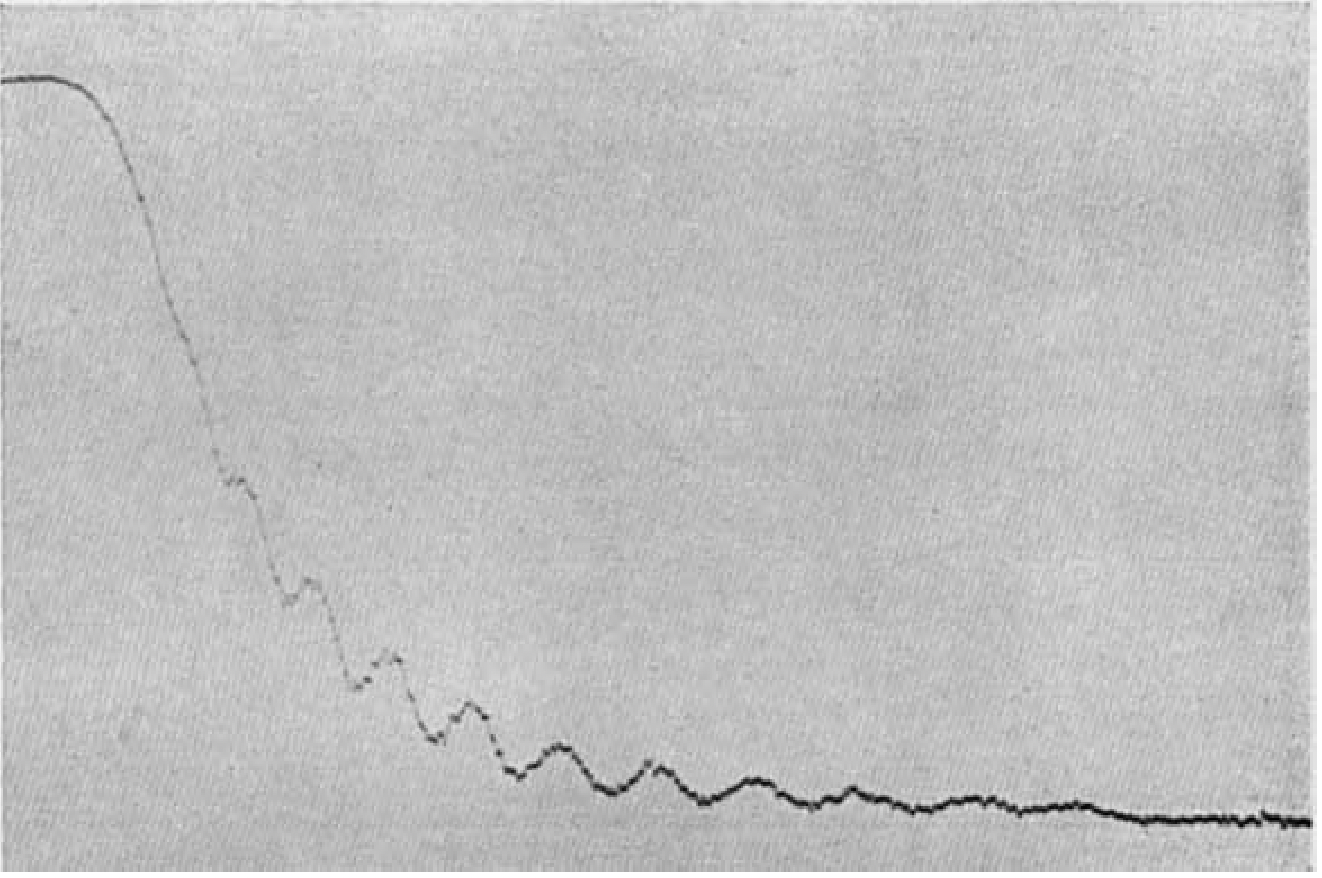
\includegraphics[width=12cm,keepaspectratio]{kiessing_oszillationen.png}
  \caption{Photometerkurve der Röntgenreflektivität eines Nickelspiegels als Funktion des Eingangswinkels.\cite{kiessig}}
  \label{fig:kiessig}
\end{figure}
In \autoref{fig:kiessig} ist eine Photometeraufnahme zu sehen, die die Reflektivität eines Nickelspiegels darstellt. Dieser besteht aus einem dünnen Nickelniederschlag auf einer Glasunterfläche. Hierbei sind Oszillationen der Reflektivität zu beobachten. Diese sogenannten Kiessig-Oszillationen kommen dadurch zustande, dass ein Teil des am ersten Medium transmittierten Strahlungsanteils am zweiten Medium reflektiert wird, welcher dann mit dem am ersten Medium reflektierten Teilstrahl interferiert. Mit Hilfe der Kiessig-Oszillationen lässt sich über die Gleichung
\begin{equation}
  d = \frac{\lambda}{2 \Delta \alpha_\mathrm{i}}
  \label{eqn:abstandoderso}
\end{equation}
die Dicke der Schicht bestimmen, wobei $\lambda$ die Wellenlänge der Strahlung ist und $\Delta \alpha_\mathrm{i}$ dem Abstand zweier Extrempunkte mit gleichem Vorzeichen entspricht.

Bei Systemen aus mehr als zwei Schichten werden die Oszillationen überlagert. Zur Quantisierung dieser Überlagerung dient der Parratt-Algorithmus \cite{parratt}. Hierbei handelt es sich um einen rekursiven Algorithmus zur Beschreibung eines Systems mit N Grenzschichten $z_\mathrm{j}$ mit der Rekursionsformel
\begin{equation*}
  X_\mathrm{j} = \frac{R_\mathrm{j}}{T_\mathrm{j}} = \exp \left( -2 i k_\mathrm{z,j} z_\mathrm{j} \right) \frac{ r_{\mathrm{j,j}+1} + X_{\mathrm{j}+1} \exp \left( 2i k_{\mathrm{z,j}+1} z_\mathrm{j} \right) }{ 1 + r_{\mathrm{j,j}+1} X_{\mathrm{j}+1} \exp \left( 2i k_{\mathrm{z,j}+1} z_\mathrm{j} \right) },
\end{equation*}
wobei $r_{\mathrm{j,j}+1}$ die Fresnelreflektivität der j-ten Grenzschicht und $k_{\mathrm{z,j}} = \sqrt{n_\mathrm{j}^2 - \cos^2 \alpha_\mathrm{i}} $ die z-Komponente des Wellenvektors in der j-ten Schicht ist.
Da die durch die letzte Grenzschicht $z_\mathrm{N}$ transmittierte Strahlung $T_{\mathrm{N}+1}$ nicht weiter reflektiert wird, gilt $R_{\mathrm{N}+1} = X_{\mathrm{N}+1} = 0$, wobei es sich um den Startwert der Rekursion handelt. Dies beruht auf der Annahme, dass die $(\mathrm{N}+1)$-te Schicht (das Substrat), genau wie die erste Schicht (das Vakuum) als unendlich angenommen wird.

Um den Parratt-Algorithmus auch auf Multischichtsysteme anzuwenden, deren Oberflächen nicht als glatt angenommen werden, müssen die Fresnel-Koeffizienten modifiziert werden. Hierzu wird zunächst die \textit{root-mean-square}-Rauigkeit
\begin{equation*}
  \sigma_\mathrm{j}^2 = \int \left( z - z_\mathrm{j} \right)^2 P_\mathrm{j} (z) dz
\end{equation*}
eingeführt, wobei $z_\mathrm{j}$ die Position der j-ten Grenzschicht und $P_\mathrm{j} (z)$ die Wahrscheinlichkeit, dass sich die j-te Grenzschicht im Intervall $[z_\mathrm{j} + z, z_\mathrm{j} + z + \mathrm{d}z]$ befindet, ist. Bei Letzterem handelt es sich um eine Gauss-Glockenfunktion der Breite $\sigma_\mathrm{j}$. Die modifizierten Fresnel-Koeffizienten sind dann gegeben durch
\begin{align*}
  \tilde{r}_{\mathrm{j,j}+1} &= r_{\mathrm{j,j}+1} \exp \left( -2 k_\mathrm{z,j} k_{\mathrm{z,j}+1} \sigma_\mathrm{j}^2 \right) &
  \tilde{t}_{\mathrm{j,j}+1} = t_{\mathrm{j,j}+1} \exp \left( \frac{ \left( k_\mathrm{z,j} - k_{\mathrm{z,j}+1} \right)^2 \sigma_\mathrm{j}^2 }{2} \right)
\end{align*}
und können anstatt der normalen Fresnel-Koeffizienten in den Parratt-Algoritmus eingefügt werden.

\subsection{Korrektur durch Geometriefaktor}
Für Einfallswinkel unter einem Grenzwinkel $\alpha_\mathrm{g}$ trifft nicht die gesamte Strahlbreite $d_0$ des Röntgenstrahls auf die Oberfläche der Probe. Für den Grenzwinkel gilt im Allgemeinen
\begin{equation*}
  \alpha_\mathrm{g} = \arcsin \left( \frac{d_0}{D} \right),
\end{equation*}
wobei $D$ die Länge der Probe ist. Um diesen Effekt zu korrigieren, wird der sogenannte Geometriefaktor
\begin{equation}
  G = \left\{
  \begin{array}{ll}
    \frac{D \sin \alpha_\mathrm{i}}{d_0} & \mathrm{für }\  \alpha_\mathrm{i} < \alpha_\mathrm{g}\\
    1 & \mathrm{für }\  \alpha_\mathrm{i} \geq \alpha_\mathrm{g} \\
\end{array}
\right.
  \label{eqn:geofaktor}
\end{equation}
eingeführt. Dabei ist $D \sin \alpha_\mathrm{i}$ die effektive Strahlbreite.
